% Copyright (C) 2007 Technical University of Liberec.  All rights reserved.
%
% Please make a following refer to Flow123d on your project site if you use the program for any purpose,
% especially for academic research:
% Flow123d, Research Centre: Advanced Remedial Technologies, Technical University of Liberec, Czech Republic
%
% This program is free software; you can redistribute it and/or modify it under the terms
% of the GNU General Public License version 3 as published by the Free Software Foundation.
%
% This program is distributed in the hope that it will be useful, but WITHOUT ANY WARRANTY;
% without even the implied warranty of MERCHANTABILITY or FITNESS FOR A PARTICULAR PURPOSE.
% See the GNU General Public License for more details.
%
% You should have received a copy of the GNU General Public License along with this program; if not,
% write to the Free Software Foundation, Inc., 59 Temple Place - Suite 330, Boston, MA 021110-1307, USA.

\setcounter{page}{2}

\section*{Flow123D}

\subsection*{Introduction}
Flow123D is a software for simulation of water flow, solute transport and sorption in a heterogenous 
porous and fractured medium. In particular it is suited for simulation of underground processes in a granite rock masive.
The program is able to describe explicitely processes in 3D medium, 2D fractures, and 1D chanels and exchange between those dimensions.
The computational mesh is therefore collection of 3D tetrahedrons, 2D trinagles and 1D line segments.

The water flow model assumes a saturated medium described by Darcy law. For discretization we use mixed hybrid FEM. This version
allows only calculation of steady water flow. 

The solute transport model can deal with several dissolved substances. It contains non-equilibrium dual porosity model, 
i.e. exchange between mobile and immobile 
pores. There is also model for several types of sorption in both the mobile and immobile zone. The imlemented sorption models are
linear sorption, Freundlich isotherm and Langmuir isotherm. The solute transport model uses finite volume discretization 
with upwinding in space and explicit Euler discretization in time. The dual porosity and the sorption are introduced into transport by operator spliting.
The dual porosity model use analytic solution and the non-linear adsorption is solved numerically by the Newton method.

The program is implemented in C/C++ using essentialy PETSC library for linear algebra. The water flow as well as the transport simulation can be computed 
in parallel using MPI environment. This version also support output into VTK format, which is widely supported. In particular we recommend Paraview for 
visualization and postprocessing of the results.

The program is distributed under GNU GPL v. 3 licence and is available on the project web page:
http://dev.nti.tul.cz/trac/flow123d

\subsection*{Usage}
On the Linux system the program can be started either directly or through a script \verb'run_flow.sh'. When started directly by command
\begin{verbatim}
  > flow123d -s example.ini
\end{verbatim}
the program accepts one argument after swith \verb'-s' which is the name of the principila input file. When you want to start a parallel job
you shloud rather use starting script. Basic usage is:
\begin{verbatim}
  > run_flow.sh -np 2 -s example.ini
\end{verbatim}
which run simulation on 2 processes using the same INI file as before. For other possible arguments see the begining of the script.

On the Windows system you can start a squential run by command:
\begin{verbatim}
  > flow123d.exe -s example.ini
\end{verbatim}
or a parallel run by command:
\begin{verbatim}
  > mpiexec.exe -np 2 flow123d.exe -s example.ini
\end{verbatim}



The principial input file of the program is an INI file which contains names of other necesaryinput files.
Those are the file with calculation mesh (\verb'*.msh'), the file with specification of neigbourings between dimensions (\verb'*.ngh'),
the file with material description (\verb'*.mtr') and the file with boundary conditions for the water flow problem (\verb'*.bcd').

In the case of transport simulation one have to specify also the file with transport boundary conditions (\verb'*.tbc') 
and the file with transport initial condition
for individual substances (\verb'*.tic').

 \begin{figure}[h]
    \begin{center}
      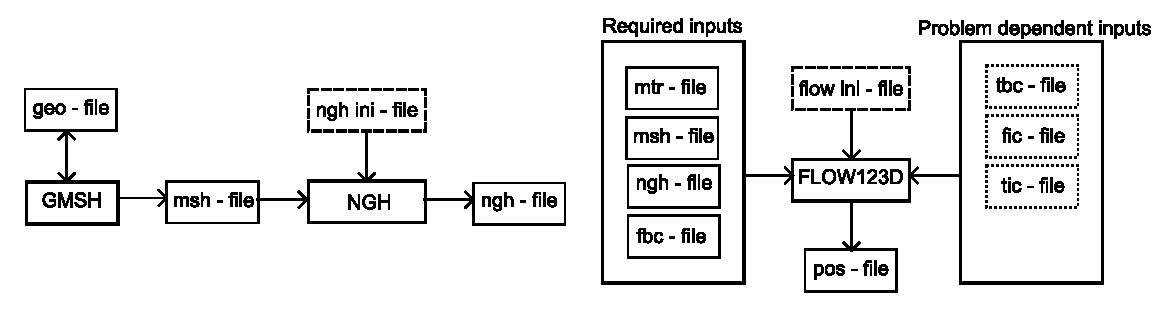
\includegraphics[scale=0.7]{schema.pdf} % 
      \caption{Preparation of input files.}
      \label{obr3}
    \end{center}
  \end{figure}


For the preparation of input files we use several utitlities (see Figure \ref{obr3}). 
We usualy begin with a \verb'*.geo' file as a description of the domain geomery. This come as an input for the GMSH mesh generator, which produce 
the mesh file. Then we run program \verb'ngh' to produce file of neigbourings. Finally we can use program \verb'bcd' for the preparation of files with
boundary and initial conditions. The file with material properties has to be created manualy, preferably by modifying some of the example problems.
The programs \verb'ngh' and \verb'bcd' are distributed together with flow123d with their own limited documentation.

The output files can be either \verb'*.pos' files accepted by the GMSH or one can use VTK format that can be postprocessed by Paraview.

In following sections we briefly describe structure of individual input files.

